%====================================================
%
% Author: PR. XAVIER NOUMBISSI NOUNDOU
%
%====================================================
\documentclass[a4paper, 12pt]{report}
\NeedsTeXFormat{LaTeX2e}
\makeindex

%---------------------------- PACKAGE INCLUSION -------------------------------
% This group renders characters clearer and more precise

\RequirePackage[bitstream-charter,cal,expert]{mathdesign}
\RequirePackage{makeidx}
\RequirePackage{latexsym}

\usepackage[numbib]{tocbibind}

\usepackage{geometry}
\geometry{a4paper,
		  %showframe=true,
		  %margin=2.75em,
		  %a4paper,
		  %total={170mm,257mm},
		  top=4.3em,
		  left=3em,
		  right=3em,
		  bottom=3.39em
		  }

\usepackage{graphicx}  

\usepackage{multicol}  	  

\usepackage{caption}

\usepackage[default]{cantarell}
\usepackage{graphicx}
\usepackage{xspace}
\usepackage[parfill]{parskip} % Activate to begin paragraphs with an empty line rather than an indent
\usepackage{paralist} % very flexible & customisable lists (eg. enumerate/itemize, etc.)
\usepackage{listings} % for lstset definitions
\usepackage{url}
\usepackage{subfig} % make it possible to include more than one captioned figure/table in a single float
\usepackage{epsfig}
\usepackage{booktabs}
%\usepackage{enumitem} %funny itemize icons
\usepackage{verbatim}
\usepackage{tcolorbox}

\usepackage{pagecolor}

\usepackage{amsmath}
\newcommand{\mathbold}[1]{\text{\textbf{#1}}}

\usepackage{xcolor}
\definecolor{yerothColorOrange}{RGB}{242, 161, 0}   
\definecolor{yerothColorBlue}{RGB}{77 , 93 , 254}
\definecolor{yerothColorRed}{RGB}{254, 48 , 48}
\definecolor{yerothColorGray}{RGB}{198, 198, 198}
\definecolor{yerothColorDarkgray}{RGB}{60, 60 , 60}
\definecolor{yerothColorIndigo}{RGB}{83, 0, 125}
\definecolor{yerothColorGreen}{RGB}{2  , 160, 70}
\definecolor{forestgreen}{RGB}{2,160,70}    
\definecolor{mediumblue}{RGB}{7,43,205}    
\definecolor{firebrickred}{RGB}{178,34,34}
\definecolor{listingray}{gray}{0.9}
\definecolor{lbcolor}{rgb}{0.9,0.9,0.9}
\definecolor{darkgreen}{rgb}{0,0.35,0}
\definecolor{medgreen}{rgb}{0,0.5,0}
\definecolor{lightgreen}{rgb}{0.5,0.7,0.5}
\definecolor{pmcolour}{rgb}{0.5,0.7,0.5}
\definecolor{medgrey}{rgb}{0.6,0.6,0.6}
\definecolor{purplish}{rgb}{0.4,0,0.6}
\definecolor{brightred}{rgb}{1,0.2,0.2}

\newcommand{\diplinfn}{DR.\xspace}

\newcommand{\yerothrd}{\textcolor{yerothColorGreen}
			{\textsc{\textcolor{yerothColorRed}{YEROTH}}$_{\text{r\&d}}$\xspace}}

\newcommand{\mytime}[2]{$#1$:$#2$\xspace}

\newcommand{\debianlinux}{\texttt{Debian--Linux}\xspace}

\newcommand{\webbrowserbased}{web--browser--based\xspace}

\newcommand{\yerotherpblack}{YEROTH--ERP--$3.0$\xspace}

\newcommand{\yerotherp}{\textsc{\textcolor{yerothColorBlue}{YEROTH--ERP--$3.0$}}\xspace}

\newcommand{\saperp}{'SAP Business One'\xspace}

\newcommand{\sageerp}{'Sage Gescom i$7$'\xspace}

\newcommand{\myfullacademicname}{PR. XAVIER NOUMBISSI NOUNDOU\xspace}

\usepackage{hyperref}
\hypersetup{
    colorlinks,
	pagebackref,
    citecolor=medgreen,
    linkcolor=purplish,
    breaklinks,
    pdftex,
    bookmarks,
    plainpages=false,
	pdftitle={\yerotherpblack | UTILISATIONS RECOMMANDÉS: R\'edig\'e
		par ''\myfullacademicname''.},
    pdfauthor={\myfullacademicname}
}

%--------------------------------------------------------------------------------

%---------------------------- COMMANDS DEFINITION -------------------------------
\newcommand{\diplinf}{\emph{Dipl.-Inf.}\xspace}
\newcommand{\mycheckmark}[1]{\textcolor{#1}{$\checkmark$}\xspace}

\newcommand{\myenumitem}[1]{\emph{#1}\xspace}
\newcommand{\yerenalert}{\emph{yeren-alert}\xspace}

\newcommand{\erpsoftware}{ERP~software--system\xspace}

\newcommand{\wy}{WYSIWYG\xspace}

\newcommand{\thickclient}{thick--client\xspace}

\newcommand{\ministudio}{\texttt{miniStudio (vxWorks)}\xspace}

\newcommand{\ERPNext}{\texttt{ERPNext}\xspace}

\newcommand{\Odoo}{\texttt{Odoo}\xspace}

\newcommand{\lxqtsudo}{\texttt{lxqt--sudo}\xspace}

\newcommand{\logFourJ}{\texttt{Log$4$j}\xspace}

\newcommand{\qtdesigner}{\texttt{Qt designer}\xspace}

\newcommand{\YEROTHCHAPINTRO}[1]{
\begin{center}
\parbox{35em}{
\textcolor{yerothColorIndigo}{#1}
}\xspace
\end{center}}

\newcommand{\gplusplus}{\texttt{gcc~(g$++$)}\xspace}

\newcommand{\cplusplus}{\texttt{C$++$}\xspace}

\newcommand{\ERPNextProgrammingLanguages}{\texttt{JavaScript, Python}\xspace}

\newcommand{\OdooLibraries}{\texttt{python--lxml, etc.}\xspace}

\newcommand{\OdooProgrammingLanguages}{\texttt{Python, JavaScript, XML}\xspace}

\newcommand{\Java}{\texttt{Java}\xspace}

\newcommand{\apache}{\texttt{Apache web server}\xspace}

\newcommand{\Werkzeug}{\texttt{Werkzeug}\xspace}

\newcommand{\PostgreSQL}{\texttt{PostgreSQL}\xspace}

\newcommand{\MySQL}{\texttt{MySQL}\xspace}

\newcommand{\JBoss}{\texttt{JBoss}\xspace}

\newcommand{\unibremen}{University of Bremen}

\newcommand{\definition}[1]{\textbf{\textcolor{yerothColorBlue}{\section{#1}}}\xspace}

\newcommand{\yerothvert}[1]{\textcolor{yerothColorGreen}{#1}\xspace}
\newcommand{\yerothrouge}[1]{\textcolor{yerothColorRed}{#1}\xspace}

\newcommand{\systemelogiciel}{SYST\`EME--LOGICIEL\xspace}

\newcommand{\featuresummary}[2]{\textbf{\textcolor{#1}{\textsc{#2}}}}

%--------------------------------------------------------------------------------

\usepackage[T1]{fontenc}
\newcommand{\changefont}[3]{
\fontfamily{#1} \fontseries{#2} \fontshape{#3} \selectfont}
\changefont{cmss}{m}{n}

\renewcommand\labelenumi{\theenumi)}

\pagenumbering{arabic}

%%%%%%%%%%%%%%%%%%%%SETTING HEADER AND FOOTER FOR 'REPORT CLASS'.%%%%%%%%%%%%%%%%%%%%%
\usepackage{fancyhdr}
\pagestyle{fancy}
\renewcommand{\headrulewidth}{0pt}
\fancyhf{}

\fancypagestyle{plain}{% copies "fancy" over "plain"
  \fancyfoot[C]{\thepage}% you can add edits that won't affect "fancy" but only "plain"
}

\fancypagestyle{OnlyFirstPage}{%
	\lhead{}
	\rhead{}
    \lfoot{}
}

\rhead{\yerotherpblack Software--System Architecture}
\lhead{\textbf{\yerothrd}}
\lfoot{}
\rfoot{}
\cfoot{\thepage}


%%%%%%%%%%%%%%%%%%%%%%%%%%%%%%%%%%%%%%%%%%%%%%%%%%%%%%%%%%%%%%%%%%%%%%%%%%%

\clubpenalty = 10000
\widowpenalty = 10000
\displaywidowpenalty = 10000

\pdfminorversion=7

\begin{document}

\thispagestyle{OnlyFirstPage}

{\bf \Large \yerothrd} {| \sc \scriptsize \yerotherpblack guide pratique du SYSTÈME--LOGICIEL YEROTH-ERP-3.0}
\\ \line(1,0){540}

\vspace{2.0em}

\begin{center}
{\LARGE \yerotherpblack | GUIDE PRATIQUE}
\end{center}

\vspace{2.0em}

\begin{center}
{\large \myfullacademicname}
\end{center}

\vspace{4.0em}

\begin{center}
\parbox{42em}{
This document describes the \thickclient
software--system architecture of \yerotherpblack.
This document also explains the reasons for
which we chose to design and implement
\yerotherpblack as a \thickclient software--system,
as opposed to currently more popular
\webbrowserbased software--system.
\newline

\textcolor{purplish}{
This document futher demonstrates the superiority,
in terms of simplicity, speed, maintainance, and
low costs of development of \thickclient
software--system architectures over \webbrowserbased
software--system architectures !}
}
\end{center}

% TABLE OF CONTENTS
\phantomsection
%\addcontentsline{toc}{chapter}{\contentsname}
\begingroup
\tableofcontents
\endgroup

% LIST OF FIGURES
\phantomsection
%\addcontentsline{toc}{chapter}{\listfigurename}
\begingroup
\color{medgreen}
\listoffigures
\endgroup

% LIST OF TABLES
\phantomsection
%\addcontentsline{toc}{chapter}{\listtablename}
\begingroup
\color{medgreen}
\listoftables
\endgroup

\cleardoublepage

\chapter{Introduction}

\section{Motivation}

\yerotherpblack is an \textbf{Enterprise Resource Planing (ERP)}
software--system that aims 'effectiveness' and 'simplicity',
compared to other high ranked ERP software--systems
(e.g.: \sageerp, \saperp, etc.).

We chose to design and implement \yerotherpblack as
a \thickclient software--system because of the
following reasons:

\begin{enumerate}[1.]

	\item the implementation language \cplusplus
		offers much flexibility (use of macro, 
		multiple inheritance, etc.).
		
		\emph{The drawback of the multiple inheritance
		feature of \cplusplus is it can sometimes
		be very difficult to build it using "\gplusplus" !}
		
	\item the availability of \texttt{'WHAT YOU SEE IS WHAT YOU GET'}
		(\wy) tools for fast and useful
		user interface design (e.g.: \qtdesigner~\cite{qtdesigner:2020},
		\ministudio~\cite{miniStudio:2020}, etc.)
		
	\item the low number of logical software architecture
		layer ($2$) involved with the operation
		of a \thickclient software--system,	as opposed
		to a \webbrowserbased software--system
		(with at least a $4$ layers in its 
		logical software architecture ).
	
\end{enumerate}


\section{Thick--Client VS Web--Browser--based
	Software--System Architecture}


\begin{table*}[!htbp]
\centering
\resizebox{\textwidth}{!}{%to fit the table within the text width
\begin{tabular}{cccc} 

\multicolumn{1}{c}{}										&
Thick--client application \mycheckmark{yerothColorBlue}	& 
Web--browser--based application								\\ \hline

business code								&
		\yerothvert{user interface}			&						
		\yerothrouge{application server}	\\ \hline
		
co--related software--systems		&
		\yerothvert{$1$ (DBMS)}		&						
		\yerothrouge{at least $3$ (DBMS, web~/~application server)}	\\ \hline
						
number of logical layers									&
		\yerothvert{$2$ (client and data)}					&						
		\yerothrouge{$4$ (client, presentation, logic, and data)}\\ \hline
				
rapid prototyping (\wy tools)		&
		\yerothvert{yes}			&						
		\yerothrouge{very limited}	\\ \hline				
				
software security vulnerability										&
		\yerothvert{low ($1$ programming language)}					&					
		\yerothrouge{high (\emph{several} programming languages)}	\\ \hline

user interface 														&
		\yerothvert{all computers (GUI with \emph{BUSINESS CODE})}	&						
		\yerothvert{all computers (web--browser)}					\\ 		


\end{tabular}}
\caption{Thick--client application VS Web--browser--based application.\\}
\label{tab:thickclient-application-againts-webbrowserbased-application}
\end{table*}

\begin{center}

\includegraphics[scale=0.52]{images/yeroth-thickclient-application-two-tier-architecture.png}
\captionof{figure}{$2$--layers logical 
architecture of \thickclient software--system 
(Image copied from \cite{securityboulevarddotcom:2020}).}
\label{fig:yeroth-thickclient-application-two-tier-architecture}
\end{center}

Figure~\ref{fig:yeroth-thickclient-application-two-tier-architecture}
illustrates an example of a \thickclient
software--system with a $2$--layers
logical architecture.

\begin{center}
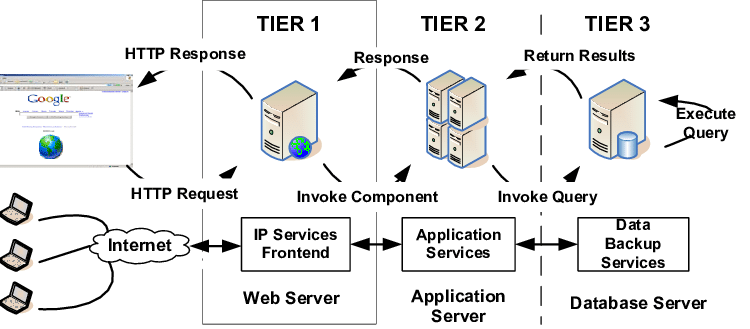
\includegraphics[scale=0.39]{images/yeroth-three-tier-architecture.png}
\captionof{figure}{$4$--layers logical architecture
of \webbrowserbased software--system
(Image copied from \cite{trevor:2006}).}
\label{fig:yeroth-three-tier-architecture}
\end{center}

Figure~\ref{fig:yeroth-three-tier-architecture}
illustrates an example of a \webbrowserbased
software--system with a $3$--layers
logical architecture.

Table~\ref{tab:thickclient-application-againts-webbrowserbased-application}
compares \thickclient software--systems against
\webbrowserbased software--systems.


\chapter{Conclusion}

\begin{table}[!htbp]
\centering
\begin{tabular}{cccc} 
\multicolumn{1}{c}{}		&
\textbf{\yerotherpblack}	&
\textbf{\Odoo} 				\\ \hline

librarires \& programs	& 	
\lxqtsudo, etc.			&	
\OdooLibraries 			\\ \hline

business code					& 	
\cplusplus						&
\OdooProgrammingLanguages		\\ \hline

DBMS 			&	
\MySQL			&
\PostgreSQL		\\ \hline

\yerothrouge{web--server}	&	
 							&
\yerothrouge{\Werkzeug}	\\ 			
\end{tabular}
\caption{\yerotherpblack VS. \Odoo VS. \ERPNext.\\}
\label{tab:Odoo-webbrowserbased-application-additional-libraries}
\end{table}
\index{\yerotherpblack VS. \Odoo \webbrowserbased software--system}

\yerotherpblack has a \thickclient
software--system architecture because we
found \thickclient software--system
architectures simpler than \webbrowserbased
software--system architectures.
\newline

Thick--client software--system architecture
are simpler because it requires less layers
in its logical software--syste architecture.
Table~\ref{tab:thickclient-application-againts-webbrowserbased-application}
illustrates a \thickclient software--system
requires less layers in its logical
software--system architecture than a
\webbrowserbased software--system.
\newline

A \webbrowserbased software--system
potentially entails more present
software security vulnerabilities 
because its implementation requires
to use at least $2$ different programming
languages, and frameworks in combination.
	
A \webbrowserbased software--system
architecture has more drawbacks as
follows:

\begin{enumerate}[1.]
	\item it requires at least $3$ other 
		software--systems, \emph{apart from
		the ones normally required by developer
		software--system itself, for instance libraries (e.g.:
		\logFourJ),} to fully operate
		(e.g.: DBMS, web server, application server.).
		
		Table~\ref{tab:Odoo-webbrowserbased-application-additional-libraries}
		depicts this situation based on the open source ERP
		software--system \Odoo.		
				
	\item A \webbrowserbased software--system
		requires at least $4$ layers in
		its logical system architecture
		(e.g.: client, presentation, logic,
		and data layers).

	\item A \webbrowserbased software--system
		potentially possesses more software
		security vulnerabilities because its
		implementation requires to use at least
		$2$ different programming languages, and
		frameworks in combination.
\end{enumerate}



\cleardoublepage
\bibliographystyle{alpha}
\bibliography{yeroth-erp-3-0-bibliography}

\cleardoublepage
\phantomsection
\printindex

\cleardoublepage
\phantomsection
\addcontentsline{toc}{chapter}{\textsc{Appendix}}
\appendix
\chapter{Commercial Presentation Documents of YEROTH--ERP--$3.0$}

\newpage

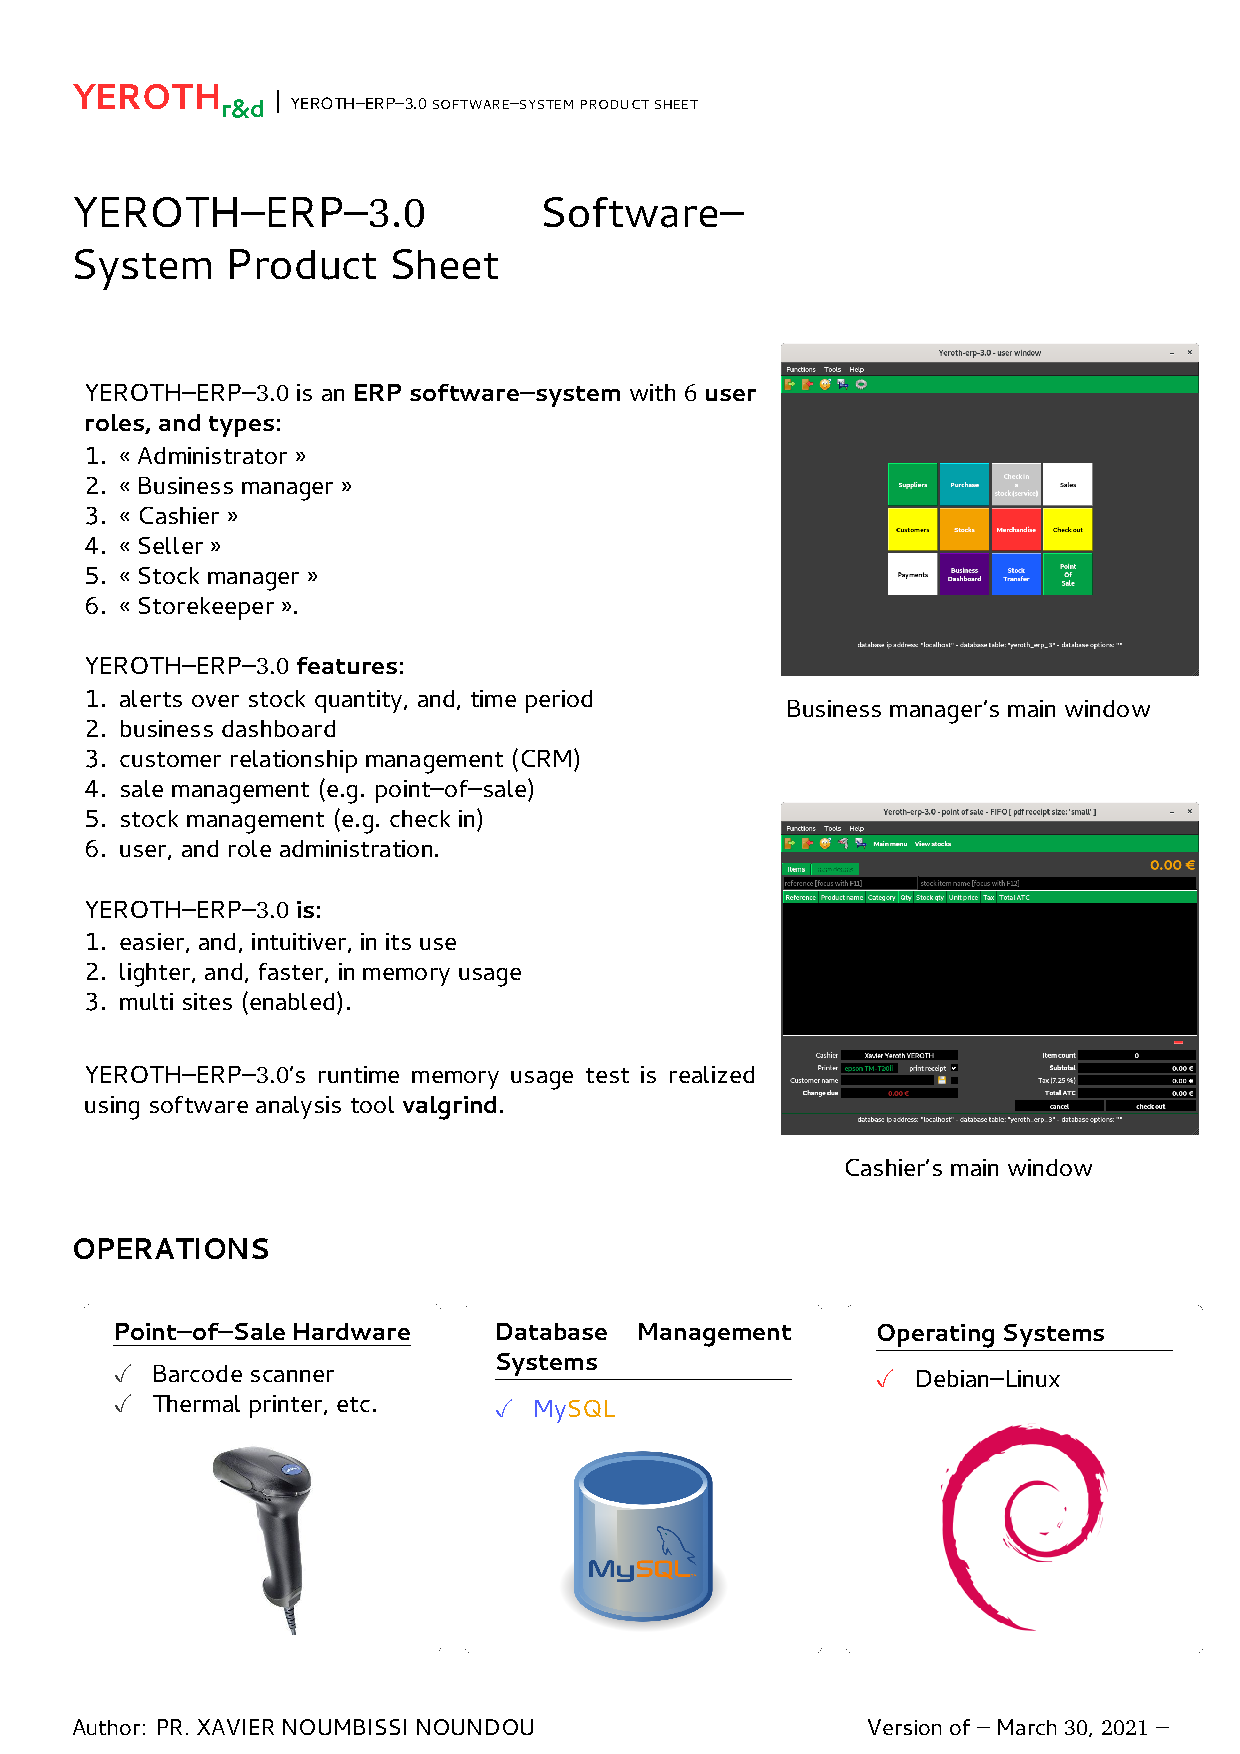
\includegraphics[scale=0.93]{../yeroth-product-sheet/yeroth-erp-3-0-product-sheet.pdf}

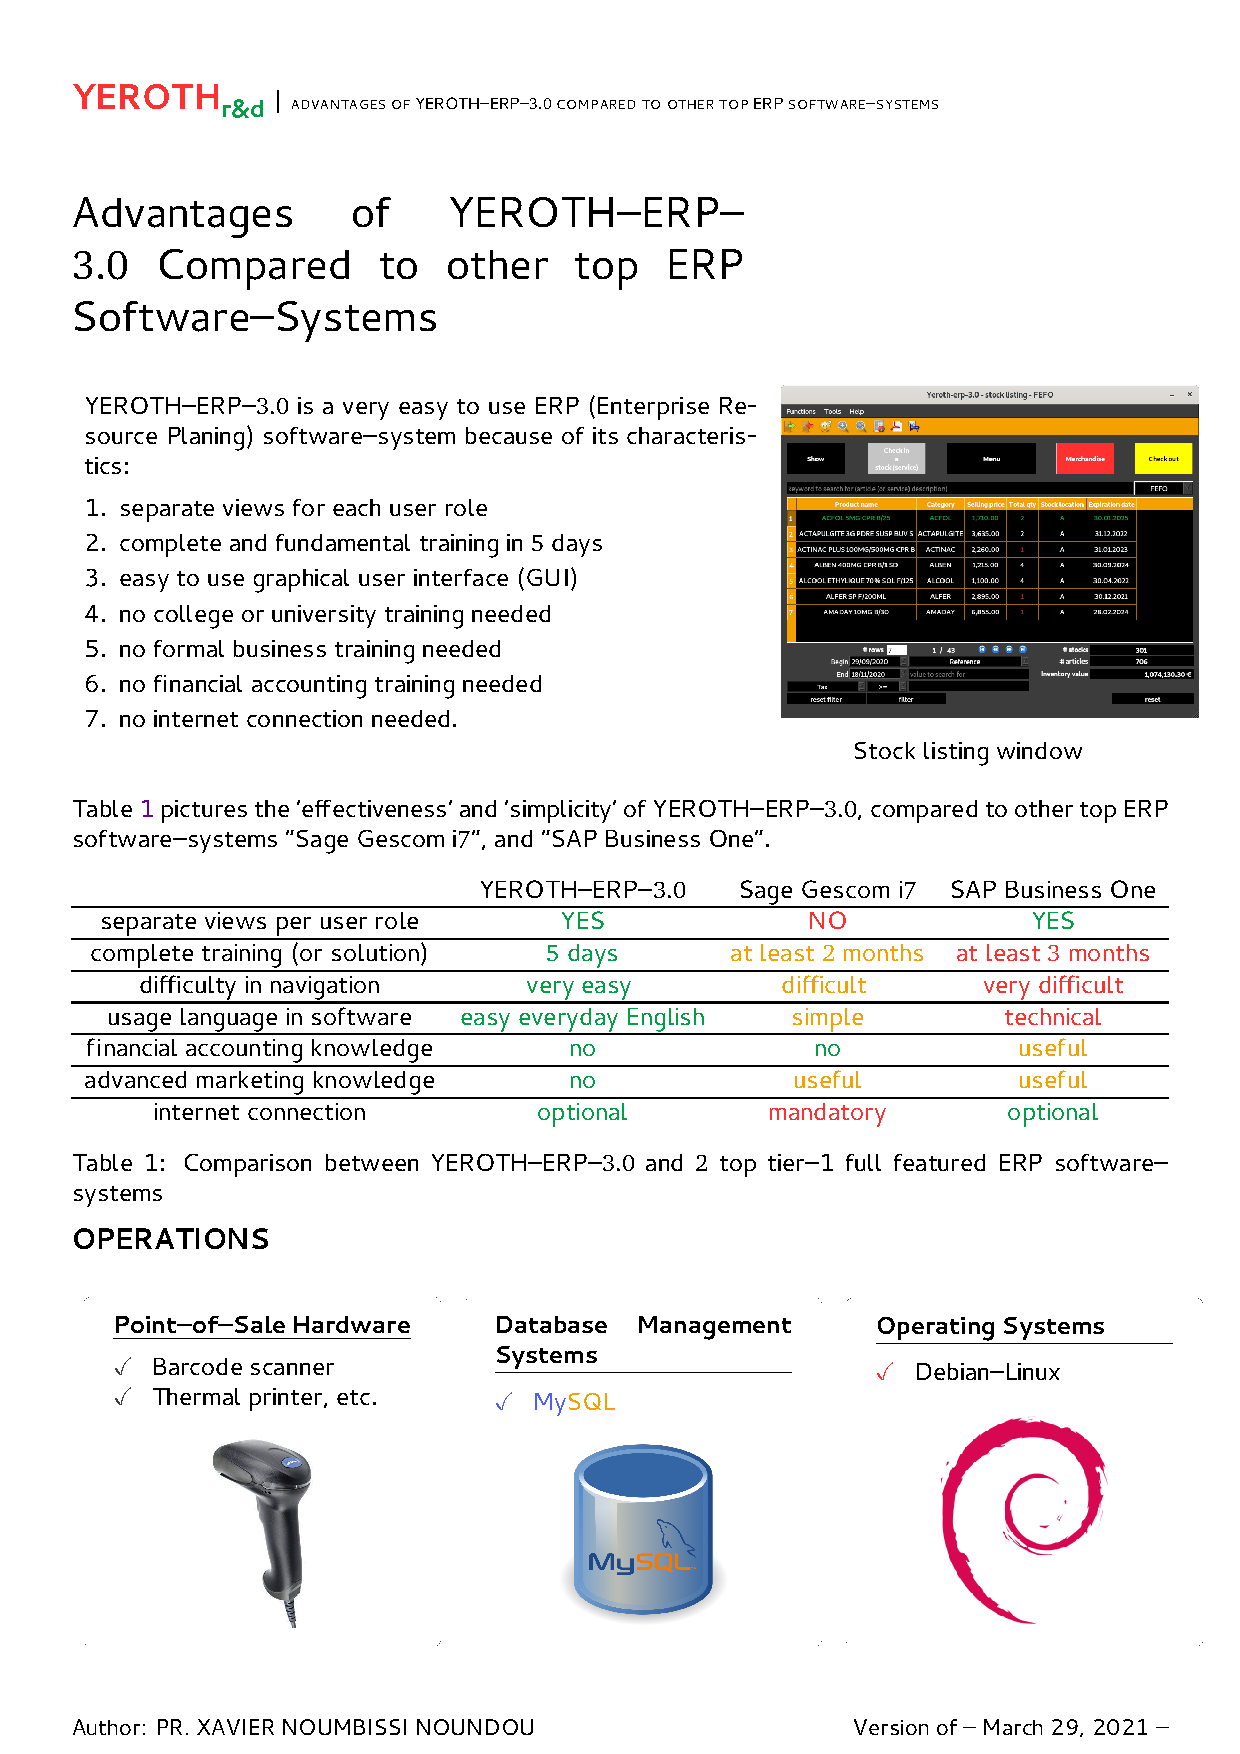
\includegraphics[scale=0.93]{../yeroth-erp-document-comparison/yeroth-erp-document-comparison.pdf}

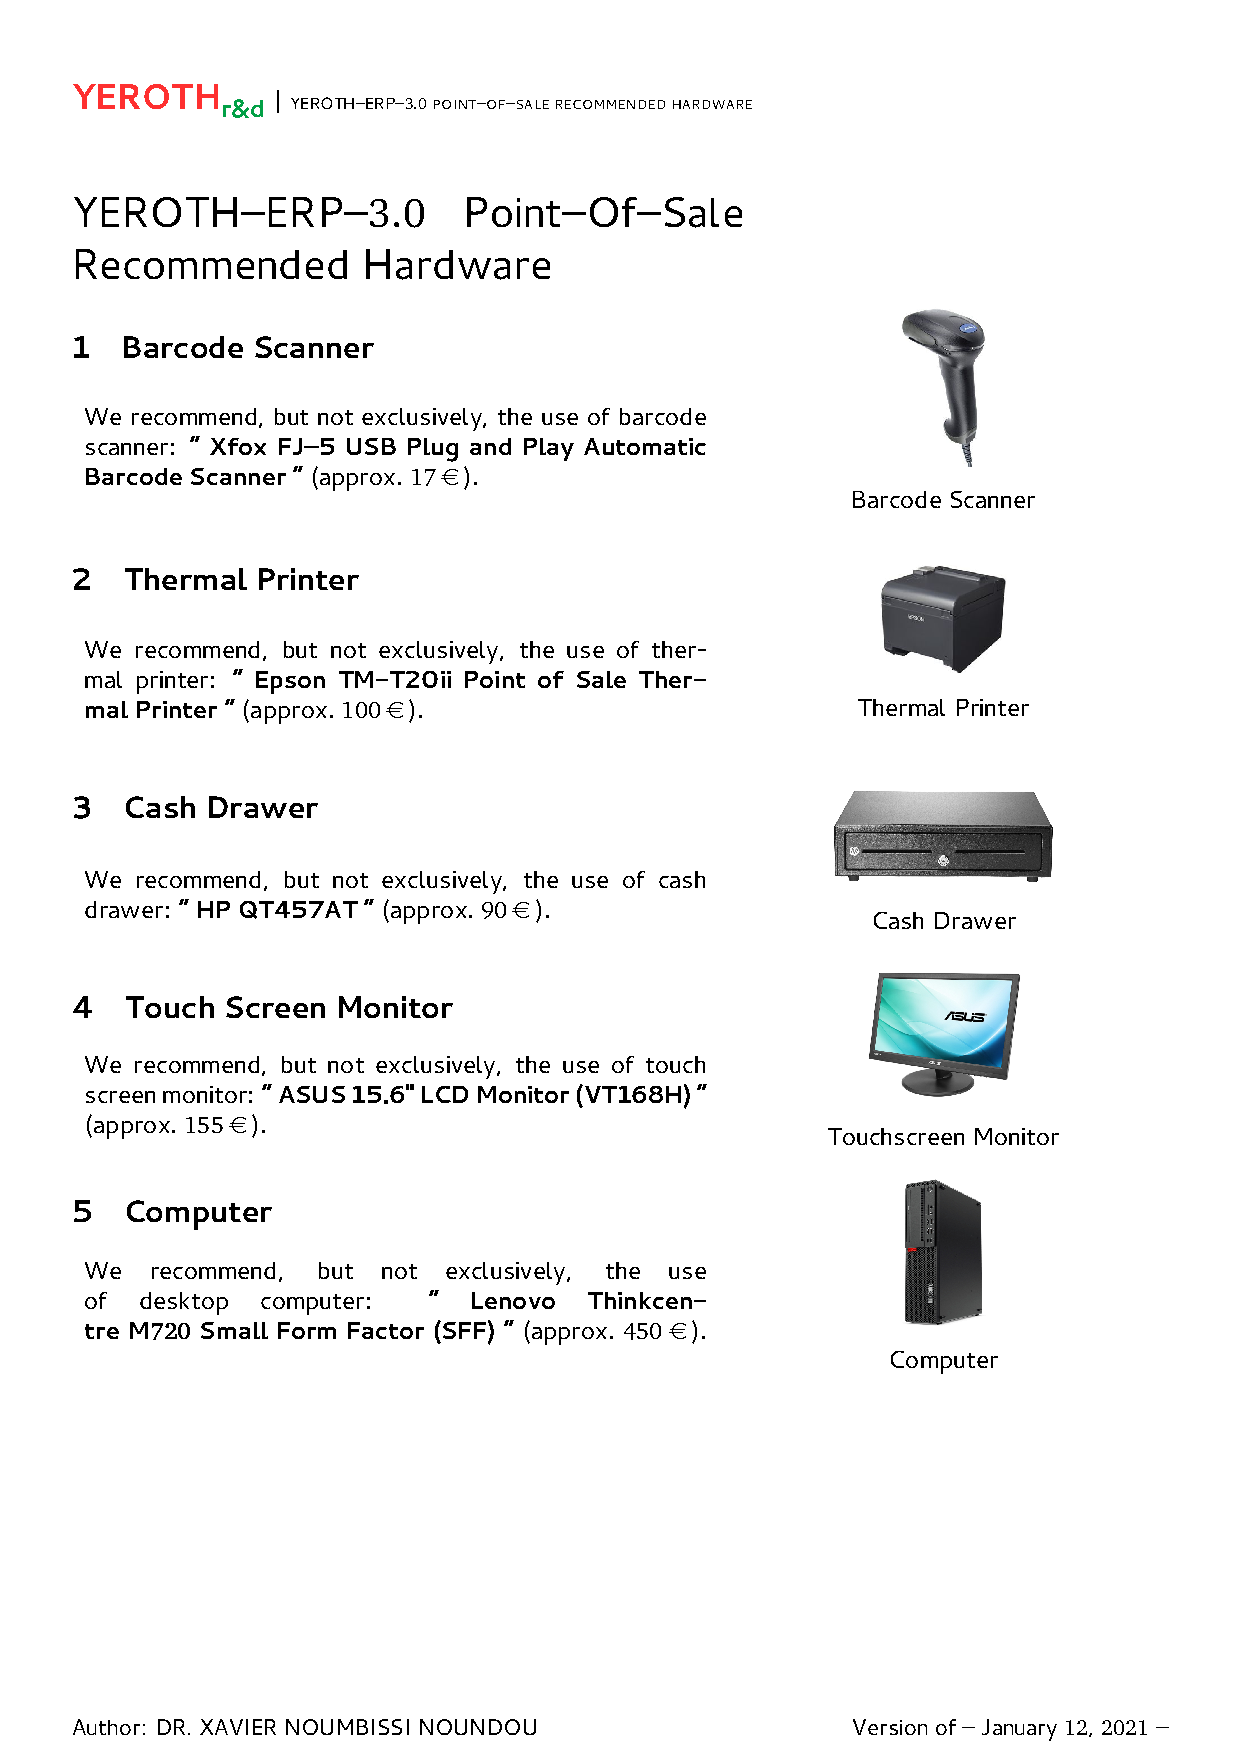
\includegraphics[scale=0.93]{../yeroth-whitepapers/yeroth-erp-3-0-inventory-stock-recommended-hardware.pdf}

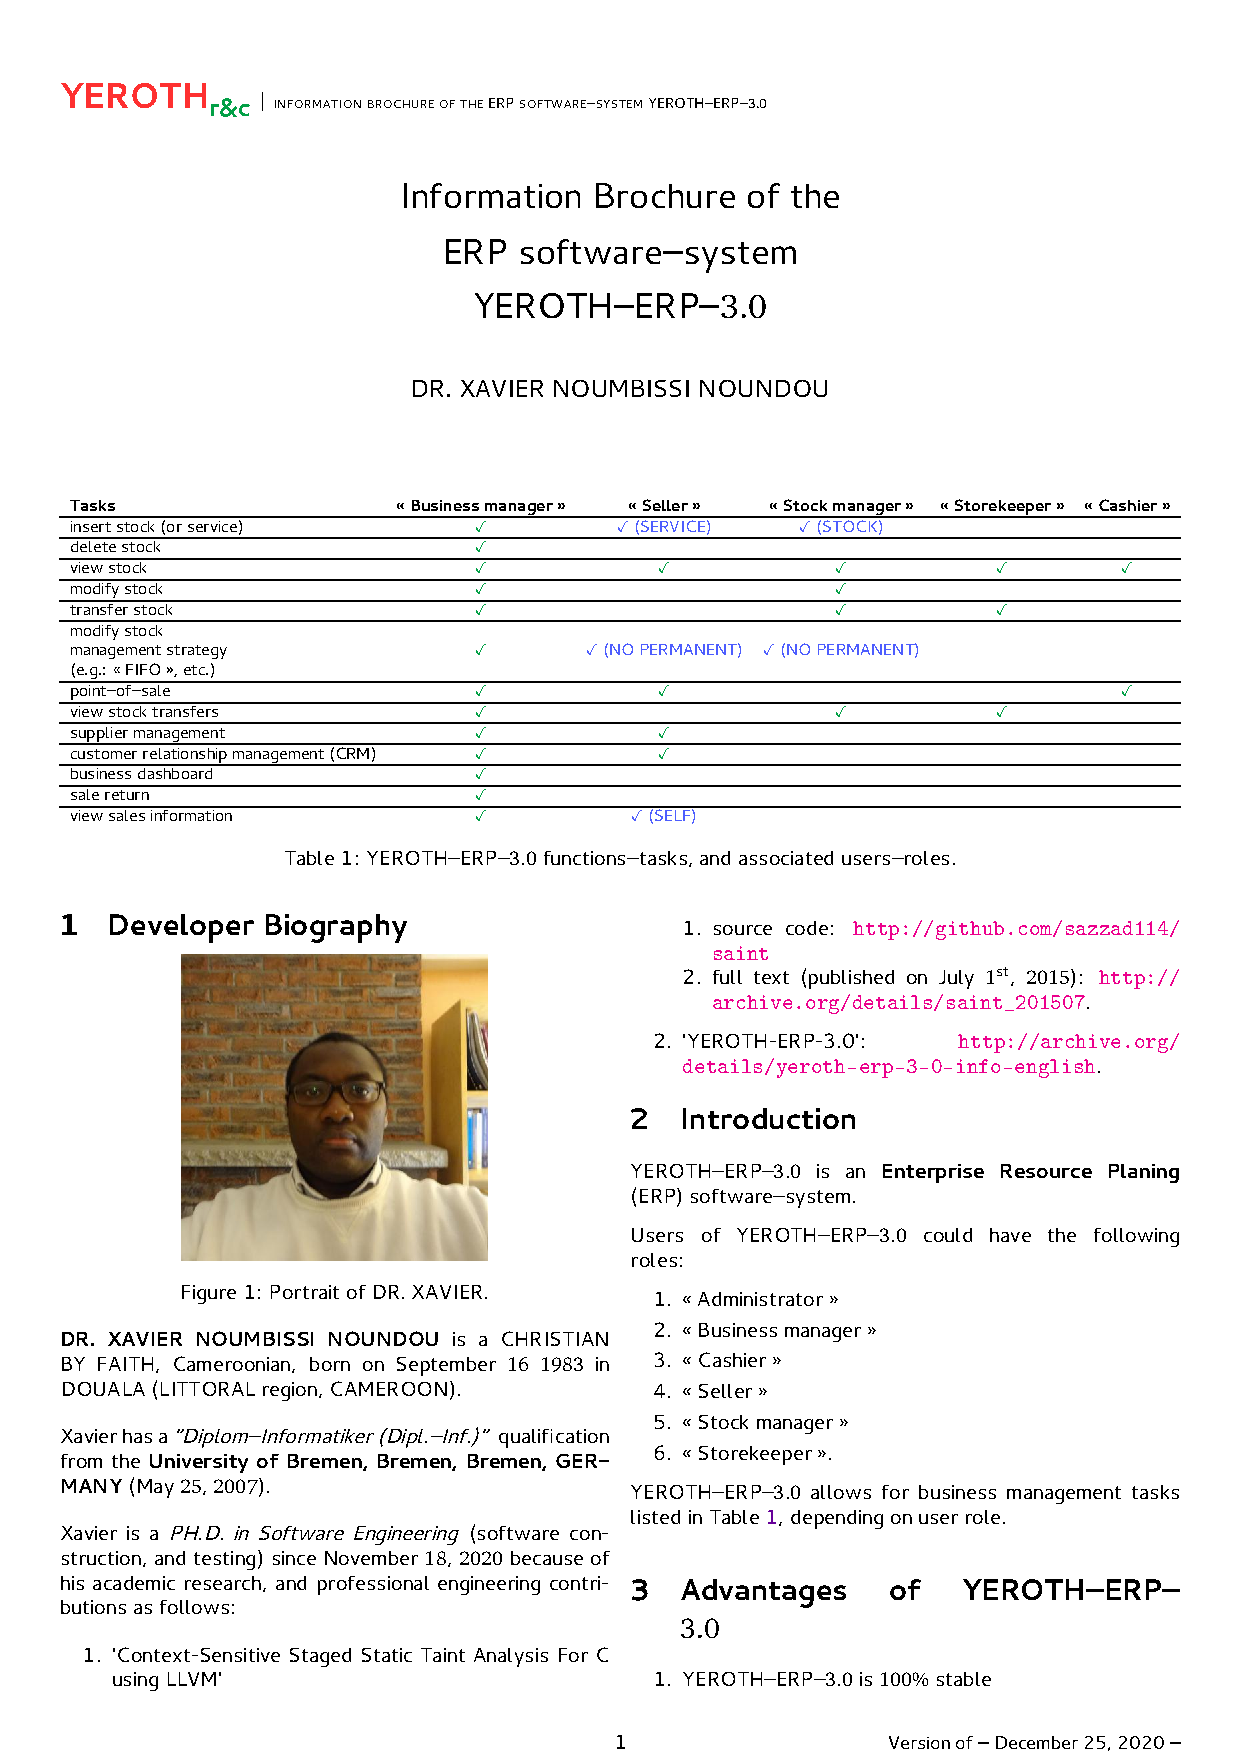
\includegraphics[scale=0.93]{../yeroth-brochure/1_yeroth-erp-3-0-brochure-english.pdf}

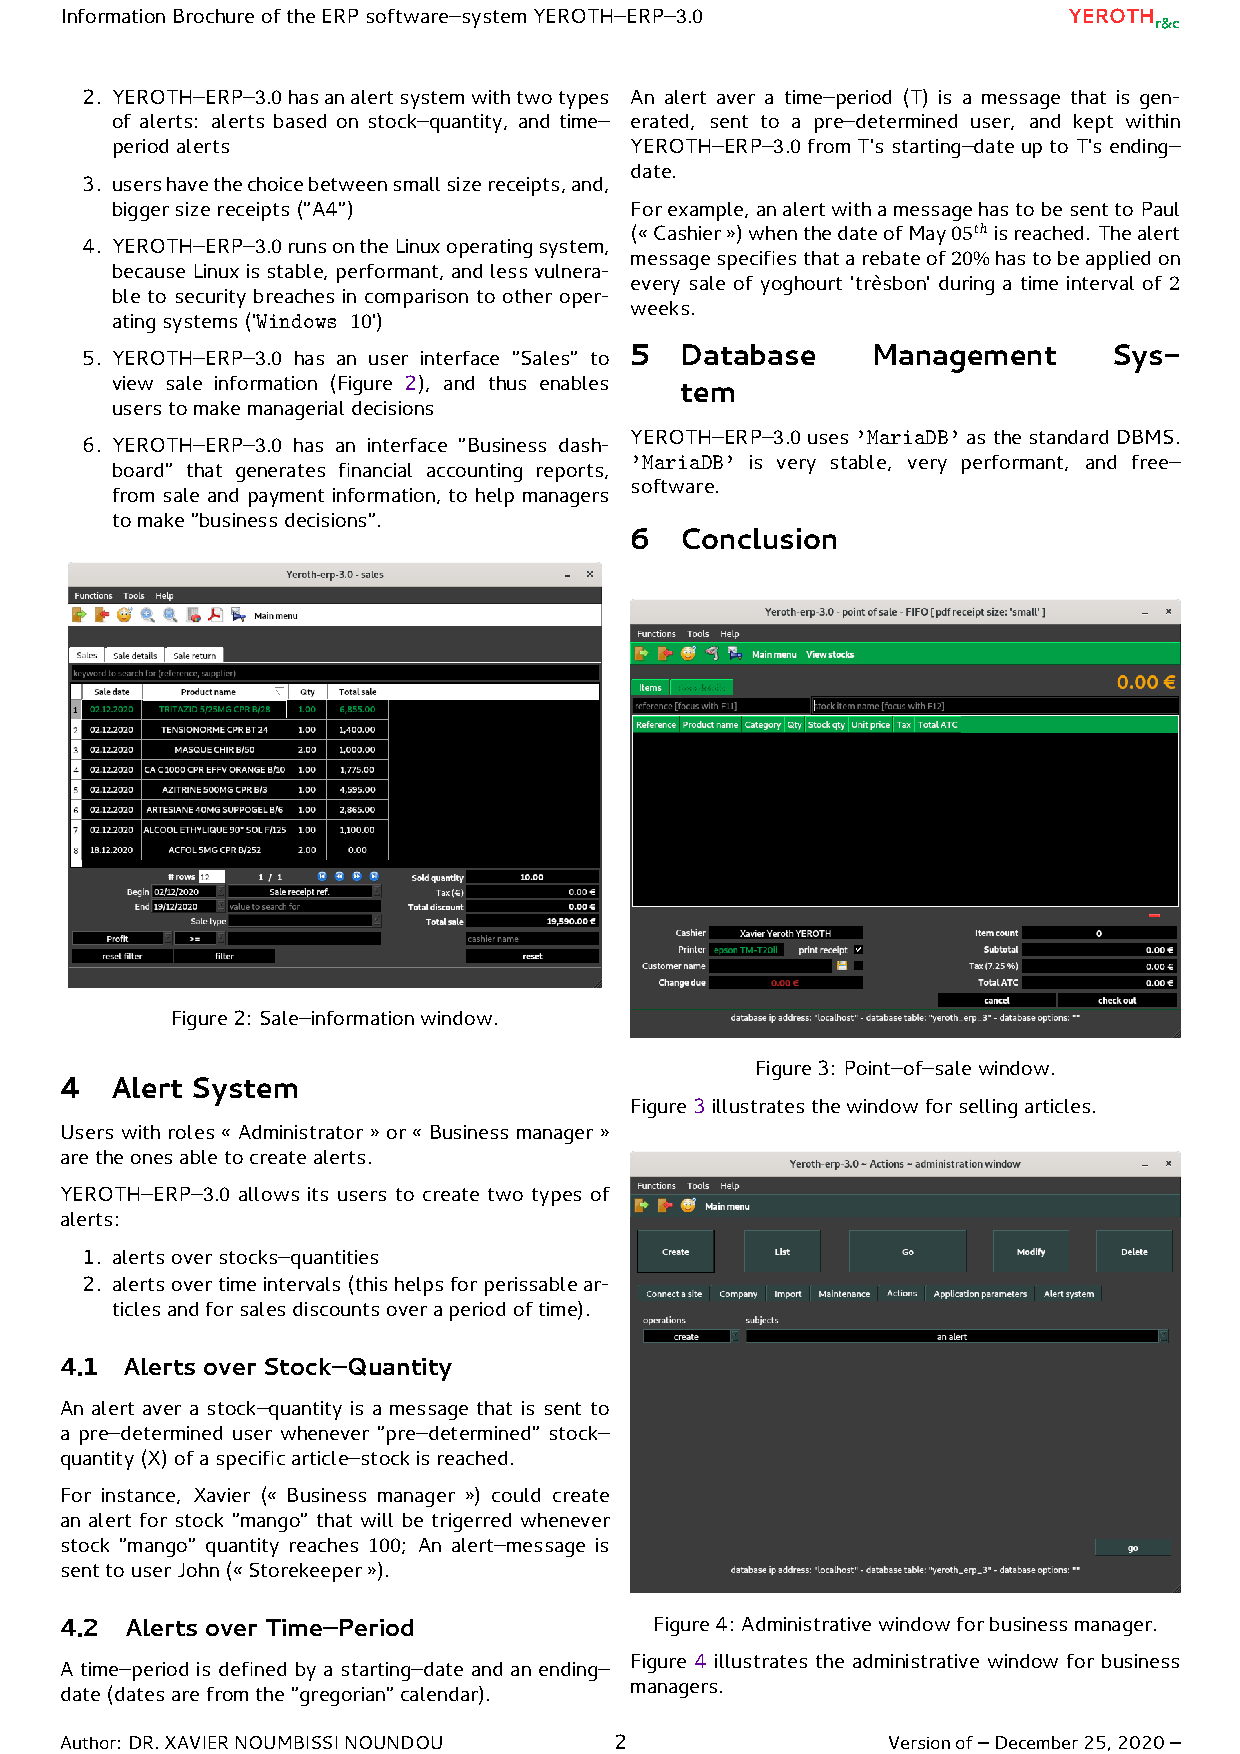
\includegraphics[scale=0.93]{../yeroth-brochure/2_yeroth-erp-3-0-brochure-english.pdf}

\end{document}

